\section{Using \padx{} to Query Ad Hoc Data}
\label{section:padx}

\begin{figure}
\begin{center}
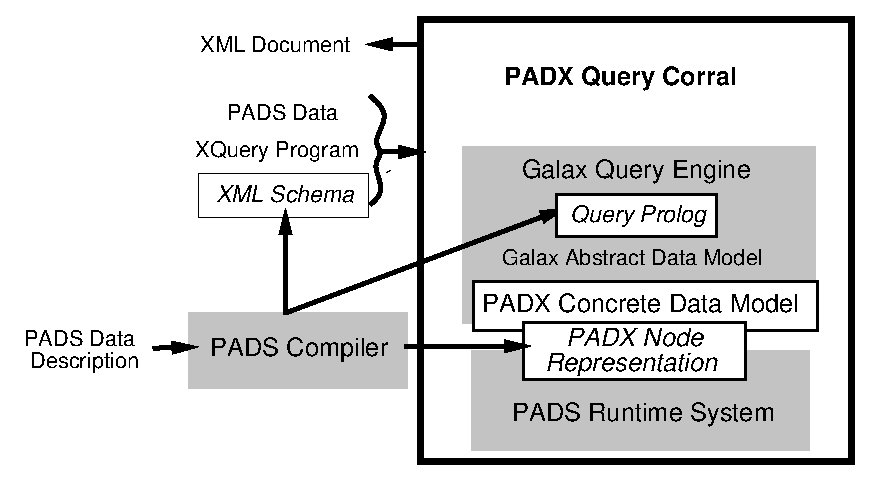
\epsfig{file=padx-arch.ps,width=0.47\textwidth}
\end{center}
\caption{\padx{} Architecture}
\label{figure:padx-arch}
\end{figure}

Put the pieces all together.  Sythesis of the two systems here. 
(Symbiotic)

\subsection{Virtual XML view of PADS data}

Embedding of PADS types in XML Schema.  One-to-one mapping from
PADS compound types to XML Schema complex types.  One-to-one mapping
from PADS base types to XML Schema simple types.  Field in compound
types are realized as local elements in XML Schema. 

All the compound types are annotated with an optional parse-descriptor
(absent if no errors occured).  Allows users to query error
structures, which may be most important data.  Other types annotated
with corresponding fields from PADS rep, e.g., arrays have a length. 

Extra level of indirection in representation of arrays---wrap each
item in an element. 

Extra level of indirection for base types: must contain the value of
the base type and an optional parse-descriptor, if an error has
occurred. 

We don't take complete advantage of XML Schema, e.g., Penum types
could be modeled by XML Schema enumeration simple types, but currently
unsupported.

Generated XML Schema.

\begin{figure*}
\begin{small}
\begin{code}
<xs:schema targetNamespace="file:sirius.p"
           xmlns="file:sirius.p"
           xmlns:xs="http://www.w3.org/2001/XMLSchema"
           xmlns:p="http://www.padsproj.org/pads.xsd">
<xs:import namespace = "http://www.padsproj.org/pads.xsd".../>
...
<xs:complexType name="\kw{order_header_t}">
 <xs:sequence>
  <xs:element name="order_num" type="p:val_Puint32"/>
  <xs:element name="att_order_num" type="p:val_Puint32"/>
  <xs:element name="ord_version" type="p:val_Puint32"/>
  <!-- More local element declarations -->
  <xs:element name="pd" type="\kw{p:PStruct_pd}" minOccurs="0"/>
 </xs:sequence>
</xs:complexType>
<!-- More complex type declarations -->
<xs:complexType name="\kw{orders_t}">
 <xs:sequence>
  <xs:element name="\kw{elt}" type="order_t" maxOccurs="unbounded"/>
  <xs:element name="\kw{length}" type="p:Puint32"/>
  <xs:element name="\kw{pd}" type="\kw{p:Parray_pd}" minOccurs="0"/>
 </xs:sequence>
</xs:complexType>
...
</xs:schema>
\end{code}
\end{small}
\caption{Fragment of XML Schema for \dibbler{} \pads{} description.}
\label{figure:dibbler-schema}
\end{figure*}

``Error-aware'' mapping from PADS type system to isomorphic XML
Schema. 
\begin{small}
\begin{code}
<xs:complexType name="\kw{val_Puint32}">
  <xs:choice>
   <xs:element name="val" type="p:Puint32"/>
   <xs:element name="pd" type="p:Pbase_pd"/>
  </xs:choice>
</xs:complexType>
<xs:complexType name="\kw{Pbase_pd}">
 <xs:sequence>
   <xs:element name="\kw{pstate}"  type="p:Pflags_t"/>
   <xs:element name="\kw{errCode}" type="p:PerrCode_t"/>
   <xs:element name="\kw{loc}"     type="p:Ploc_t"/>
 </xs:sequence>
</xs:complexType>
\end{code}
\end{small}

Example of query that uses generated schema.
\begin{small}
\begin{code}
declare namespace p = "http://www.padsproj.org/pads.xsd";
import schema default element namespace "file:sirius.p"
  schemaLocation "file:/somewhere/sirius.xsd";

$pads/p:Psource/orders/elt[events/elt[1]
  [tstamp >= xs:dateTime("2004-10-01:00:00:00") and 
   tstamp < xs:date("2004-11-01:00:00:00") ]]
\end{code}
\end{small}

\subsection{Physical Data Model}

Implementation of Galax's Abstract Tree Model.

Minimum necessary to implement Galax DM:

1. Generic implementations of the DM accessors: axis::node-test(), children(),
   attributes(), name(), etc. 

2. On PADX-side, we have a virtual handle for each node in the XML
   tree--we call that a node rep.  Node rep contains pads handle
   (maintains state for PADS parser); type-specific vtable of DM
   accessors; other stuff...

   Give example of vtable for event\_t and possibly code for
   kthChildByName. 

When to actually read from PADS data?

Options: 

1. Bulk read: Materialize entire PADS representation, populate all of the PADS
reps.  Then PADX DM lazily invoked the DM accessors over this data.
Problem: if data is big, it's all sitting in memory, even if the query
only touches a fragment of the virtual XML tree.

2. Smart read: 

Many common queries permit sequential, streamed access to underlying
XML source.  Give an example.  

Smart node rep, preserves meta-data about previously read records, but
re-uses memory for reading next item.  This rep permits multiple scans
of input (semantic problem is that DM must preserve node identity),
but slowly. 

Heuristic: records are a good level of granularity to read.   Each
smart node corresponds to one record.  When next smart node is
accessed, a little meta-data is preserved: the node rep and the
records location in the file (so we can re-read it if necessary).

3. Linear read: same as smart but does not preserve meta-data.
   Does not permit multiple scans of data source. 

Put in PADX signatures for constructing a new node and accessing
kthChild. 

